%!TEX root = ../operads_paper.tex
\section{Invertible objects}


The goal of this chapter will be to show that we can reconstruct all of the morphisms of $L_n$ from the abelian group $\MLn^{\mathrm{gp, ab}}$, and therefore that we can actually use the adjunction from \cref{Moradj} to help find a description of the free $\ML$-monoidal category on $n$ invertible objects. 

The first step towards this goal will involve splitting $\MorLn$ up as the product of two other monoids. The first of these will encode all of the possible combinations of source and target data for morphisms in $L_n$, while the second will just be the endomorphisms of the unit object, $L_n(I, I)$. 
Once we have done this, we can then use the fact that $L_n(I, I)$ is always an abelian group to rewrite $\MorLn$ in terms of its abelian group completion, $\MorLn^{\mathrm{gp, ab}}$. This is not quite the same thing as $\MLn^{\mathrm{gp, ab}}$, but they are close enough that we can find a simple equation linking the two, which will in turn allow us to frame the former in terms of the quotient of $\mathrm{M}(\ELnn)^{\mathrm{gp, ab}}$ we described last chapter. All together, this will constitute an expression for $\MorLn$ that is built up of pieces which we know how to calculate.

Current understanding is four steps:
\begin{enumerate}
\item existence of $L_n$ via adjoint functor theorem (2.1)
\item $L_n$ as a quotient of $\ELnn$ (2.2--2.3)
\item we split $L_n(I,I)$ (2.4--2.6)
\item then we make a nasty quotient (2.7 until examples)
\end{enumerate}

\subsection{Introduction to invertibility}

Our main focus will be on invertible objects, although not in the usual sense.
\begin{Defi}
Let $(M, \otimes, I)$ be a strict monoidal category. An object $m \in M$ is \emph{invertible} if there exists another object $m^{-1}$ such that $m \otimes m^{-1} = I$ and $m^{-1} \otimes m = I$.

\end{Defi}

Most authors give the following as the definition of an invertible object, what we call weakly invertible.
\begin{Defi}
Let $(M, \otimes, I)$ be a monoidal category. An object $m \in M$ is \emph{weakly invertible}\index{object!weakly invertible} if there exists another object $m^{*}$ such that $m \otimes m^{*} \cong I$ and $m^{*} \otimes m \cong I$.

\end{Defi}
We will later derive results about weakly invertible objects from those about invertible ones using standard $2$-monadic techniques.

The following lemmas describe the interaction between invertibility of objects and other aspects of the monoidal structure.

\begin{lem} \label{tenscomp} Let $f \colon  x \rightarrow y$ and $f' \colon  y \rightarrow z$ be morphisms in a strict monoidal category, and assume $y$ is an invertible object with inverse $y^{-1}$. Then
  \[
    f' \circ f \quad = \quad f' \otimes y^{-1} \otimes f
  \]
\end{lem}
\begin{proof}
By the interchange law for monoidal categories,
\begin{align*}
			f' \circ f &= (f' \otimes I) \circ (I \otimes f) \\
			&= \left(f' \otimes y^{-1} \otimes y\right) \circ \left(y \otimes y^{-1} \otimes f\right) \\
			&= \left(f' \circ \id_{y}\right) \otimes \left(\id_{y^{-1}} \circ \id_{y^{-1}}\right) \otimes (\id_y \circ f) \\
			&= f' \otimes y^{-1} \otimes f .
		\end{align*}
\end{proof} 

\begin{rem}
It is worth noting that all of the proofs which include a step described as ``an Eckmann-Hilton argument'' (see \cite{eh}) use methods similar to that above, and those are omitted from this point forward.
\end{rem}

\begin{lem}\label{inv_implies_invertible}
Let $x, y$ be invertible objects in a strict monoidal category $M$ with inverses $x^{-1}, y^{-1}$. Let $f \colon x \rightarrow y$, $g \colon x^{-1} \rightarrow y^{-1}$ be morphisms such that $f \otimes g = 1_I = g \otimes f$. Then $f, g$ are isomorphisms in $M$.
\end{lem}
\begin{proof}
The inverse of $f$ is given by 
  \[
    y = xx^{-1} y \stackrel{x \otimes g \otimes y}{\longrightarrow} xy^{-1}y = x
  \]
by an Eckmann-Hilton argument.
\end{proof}

\begin{Defi}\label{def_tensinv}
A morphism $f \colon  w \rightarrow v$ in a strict monoidal category $X$ is \emph{invertible under tensor product} or \emph{has an inverse under tensor product} if there exists another morphism $g \colon  w^{-1} \rightarrow v^{-1}$ such that $f \otimes g = \id_I = g \otimes f$; note that this requires $w, v$ to both be invertible with inverses $w^{-1}, v^{-1}$, respectively.
\end{Defi}

\begin{nota}\label{nota_tensinv}
For a morphism $f \colon w \rightarrow v$ in a strict monoidal category $X$, we write $f^*$ for its inverse under tensor product, if it exists. Standard arguments prove that $f^*$ is unique when it exists.
\end{nota}

We have the following useful converse to \cref{inv_implies_invertible}.

\begin{lem} \label{tensinv_basic} Let $f \colon  w \rightarrow v$ be an isomorphism in a strict monoidal category $X$, and assume that both $w, v$ are invertible objects. Then the inverse under tensor product $f^*$ exists.
\end{lem}
\begin{proof}
For any such $f \colon  w \rightarrow v$, consider the map $w^{-1} \otimes f^{-1} \otimes v^{-1}$, where $f^{-1}$ is the compositional inverse of $f$. This morphism has source $w^{-1}\otimes v \otimes v^{-1} = w^{-1}$ and target $w^{-1} \otimes w \otimes v^{-1} = v^{-1}$, and a simple Eckmann-Hilton argument proves that $w^{-1} \otimes f^{-1} \otimes v^{-1}$ is the tensor inverse of $f$.
% which allows us to apply the law of interchange to get
%\begin{longtable}{RLL}
%			f \otimes (\id_{w^*} \otimes f^{-1} \otimes \id_{v^*}) & = & \left( \, f \circ \id_w \, \right) \otimes \left( \, \id_{v^*} \circ  (\id_{w^*} \otimes f^{-1} \otimes \id_{v^*}) \, \right) \\
%			& = & \left( \, f \otimes \id_{v^*} \, \right) \circ \left( \, \id_w \otimes (\id_{w^*} \otimes f^{-1} \otimes \id_{v^*}) \, \right) \\
%			& = & ( f \otimes \id_{v^*} ) \circ ( f^{-1} \otimes \id_{v^*}) \\
%			& = & \id_I
%\end{longtable}
%and 
%\begin{longtable}{RLL}
%			(\id_{w^*} \otimes f^{-1} \otimes \id_{v^*}) \otimes f & = & \left( \, (\id_{w^*} \otimes f^{-1} \otimes \id_{v^*}) \circ \id_{w^*} \, \right) \otimes \left( \, \id_v \circ f \, \right) \\
%			& = & \left( \, (\id_{w^*} \otimes f^{-1} \otimes \id_{v^*}) \otimes \id_v \, \right) \circ \left( \, \id_{w^*} \otimes f \, \right) \\
%			& = & (\id_{w^*} \otimes f^{-1}) \circ (\id_{w^*} \otimes f) \\
%			& = & \id_I,
%\end{longtable}
%so $f^* := \id_{w^*} \otimes f^{-1} \otimes \id_{v^*}$ is the inverse of $f$ in the monoid $\MorLn$.
\end{proof}



\begin{Defi}\label{invdef} Given a $\ML$-monoidal category $X$, we will denote by $X_{\mathrm{inv}}$\nomenclature[N]{$X_{\mathrm{inv}}$}{the sub-$\ML$-monoidal category of $X$ of objects invertible under tensor product}\index{algebra!of weakly invertible objects} the sub-$\ML$-monoidal category of $X$ containing all objects which are invertible under tensor product, and all of the isomorphisms between them. \end{Defi} 

First note that this is indeed a well-defined $\ML$-monoidal category since the tensor product of invertible objects is again invertible, the tensor product of isomorphisms is again an isomorphism, and all of the morphisms giving the group actions are isomorphisms. The following proposition is then easily verified.

\begin{prop} \label{invprop} The assignment $X \mapsto X_{\mathrm{inv}}$ can be extended to a $2$-functor $(\_)_{\mathrm{inv}} \colon  \lmc \rightarrow \lmc$.
\end{prop}

\begin{prop} \label{invadj} The $2$-functor $(\_)_{\mathrm{inv}} \colon  \lmc \rightarrow \lmc$ has a left $2$-adjoint, $L \colon  \lmc \rightarrow \lmc$.
\end{prop}
\begin{proof} Since we already know that $\lmc$ is locally finitely presentable as an ordinary category, the conditions of the Adjoint Functor Theorem given as Theorem 1.66 in \cite{ar} amount to showing that $(\_)_{\mathrm{inv}}$ preserves both limits and filtered colimits.
\begin{itemize}
\item Given an indexed collection of $\ML$-monoidal category $X_i$, the $E\Lambda$-action of their product $\prod X_i$ is defined componentwise. In particular, this means that the tensor product of two objects in $\prod X_i$ is just the collection of the tensor products of their components in each of the $X_i$. An invertible object in $\prod X_i$ is thus simply a family of invertible objects from the $X_i$, so $(\prod X_i)_{\mathrm{inv}} = \prod (X_i)_{\mathrm{inv}}$.
\item Given $\ML$-monoidal functors $F, G \colon  X \rightarrow Z$,  the $E\Lambda$-action on their equalizer is the restriction of that on $X$. As above, this implies that an invertible object of the equalizer is merely an object of the equalizer which is invertible in $X$, so $X \mapsto X_{\mathrm{inv}}$ preserves equalizers. Combined with the previous point, taking invertible objects therefore preserves all ordinary limits.
\item Given a filtered diagram $D$ of $\ML$-monoidal categories, the $E\Lambda$-action of its colimit $\mathrm{colim}(D)$ is defined in the following way: use filteredness to find an algebra which contains (representatives of the classes of) all the things you want to act on, then apply the action in that algebra. In the case of tensor products this means that $[x]\otimes[y] = [x \otimes y]$, and thus an invertible object in $\mathrm{colim}(D)$ is just (the class of) an invertible object in one of the algebras of $D$. In other words, $\mathrm{colim}(D)_{\mathrm{inv}} = \mathrm{colim}(D_{\mathrm{inv}})$.
\end{itemize}
Thus the underlying functor of $(\_)_{\mathrm{inv}}$ has a left adjoint $L$.

To upgrade this into a $2$-adjunction, we require that $(\_)_{\mathrm{inv}}$ preserves cotensors (see \cite{borceux2} Theorem 6.7.6) over $\cat$. Let $A$ be a category and $X$ a $\ML$-monoidal category. It is straightforward to check that the cotensor $[A, X]$ is the functor category equipped with the pointwise $E\Lambda$-action. The unit object is the constant functor at $I$, the unit object of $X$;  we write this $c_I$. The cotensor $[A, X_{\mathrm{inv}}]$ consists has
\begin{itemize}
\item objects all functors $F \colon A \rightarrow X$ with the property that $Fa$ is invertible under tensor product or composition, respectively, in $X$ for all objects or morphisms, respectively, in $A$; and
\item morphisms all natural isomorphisms between them.
\end{itemize}
It is clear that $[A, X_{\mathrm{inv}}]$ is a full sub-$\ML$-monoidal category of $[A, X]_{\mathrm{inv}}$, so we check they have the same objects. If $F \otimes G = c_I = G \otimes F$ in $[A, X]$, then it is clear that $Fa$ is invertible in $X$ for every object $a \in A$. The analogous statement on the level of morphisms follows from \cref{inv_implies_invertible}.
\end{proof}

\begin{nota}\label{eta}
From this point forward, we reserve $\eta$ for the unit of the $2$-adjunction in \cref{invadj}.
\end{nota}



\begin{Defi}
Let $L_n = L\left(E\Lambda(\underline{n}) \right)$\nomenclature[C]{$L_n$}{the free $\ML$-monoidal category on $n$ invertible objects}\index{monoidal category!$\ML$-monoidal!free}, where $\underline{n} = \{x_1, \ldots, x_n \}$ is a set with $n$ elements.
\end{Defi}

\begin{thm} The algebra $L_n$ is the free $\ML$-monoidal category on $n$ invertible objects:  for any other $\ML$-monoidal category $X$, there exists an isomorphism of categories
  \[
    \lmc(L_n, X) \cong (X_{\mathrm{inv}})^n,
  \]
$2$-natural in $X$.
\end{thm}
The following $2$-natural isomorphisms arise from the adjunctions for $L$ and the free $\ML$-monoidal category monad.
\begin{align*}
		 \lmc\left( L\left(E\Lambda(\underline{n}) \right), X\right) & \cong \lmc( E\Lambda(\underline{n}), X_{\mathrm{inv}}) \\
		&\cong \cat( \underline{n}, X_{\mathrm{inv}}) \\
		&\cong X_{\mathrm{inv}}^n
\end{align*}

% QQQ Proof?

\begin{prop} \label{linveql} Let $X$ be a $\ML$-monoidal category. Then $(LX)_{\mathrm{inv}} = LX$.
\end{prop}
\begin{proof}
Let $j \colon  X_{\mathrm{inv}} \rightarrow X$ denote the obvious inclusion functor. By construction, there is an equality of functors $(\_)_{\mathrm{inv}} \circ (\_)_{\mathrm{inv}} = (\_)_{\mathrm{inv}}$ and moreover $j_\mathrm{inv} \colon  (X_\mathrm{inv})_\mathrm{inv} \rightarrow X_\mathrm{inv}$ is the identity for every $X$. Since $\lmc(LX , Y)\cong \lmc(X, Y_{\mathrm{inv}})$ is natural in $Y$, the following is a commutative square
\begin{center}
    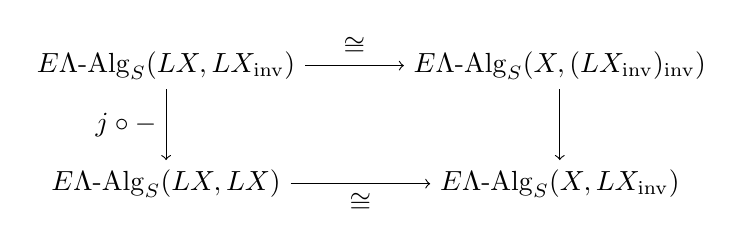
\begin{tikzpicture}[x=50mm,y=15mm]
		\node (a) at (0,0) {$E\Lambda\mbox{-}\mathrm{Alg}_S(LX , LX_{\mathrm{inv}})$};
		\node (b) at (1,0) {$E\Lambda\mbox{-}\mathrm{Alg}_S(X, (LX_{\mathrm{inv}})_{\mathrm{inv}})$};
		\node (c) at (0,-1) {$ E\Lambda\mbox{-}\mathrm{Alg}_S(LX , LX)$};
		\node (d) at (1,-1) {$E\Lambda\mbox{-}\mathrm{Alg}_S(X, LX_{\mathrm{inv}})$};
			\draw [->] (a) to node [above] {$\cong$} (b);
			\draw [->] (b) to node [right] {$\id$} (d);
			\draw [->] (a) to node [left] {$j \circ -$} (c);
			\draw [->] (c) to node [below] {$\cong$} (d);
    \end{tikzpicture}
    \end{center}
in which the identity on the right is really $j_{\mathrm{inv}} \circ -$. Thus composition with $j$ is an isomorphism in this case, so the identity map on $LX$ factors as $j \circ g$ for some $g \colon  LX \rightarrow (LX)_{\mathrm{inv}}$. Since $j$ is an inclusion, this factorization forces it to be the identity.
\end{proof}

\begin{cor} \label{epi} The component of the unit of the adjunction $L \dashv (-)_{\mathrm{inv}}$ at $E\Lambda(\underline{n})$,  $\eta_{E\Lambda(\underline{n})} \colon  E\Lambda(\underline{n}) \rightarrow (L_n)_{\mathrm{inv}}$, is an epimorphism in $E\Lambda\mbox{-}\mathrm{Alg}_S$.
\end{cor}
\begin{proof}
By \cref{linveql}, we first have that $(L_n)_{\mathrm{inv}} = L_n$. Let $F,G \colon  L_n \rightarrow X$ be a pair of algebra maps for which $F \eta = G \eta$. Thus the algebra maps $E\Lambda(\underline{n}) \rightarrow X_{\mathrm{inv}}$ corresponding to $F, G$ are equal, so $F,G$ are equal.
\end{proof}

%\begin{rem}
%include forward ref to where we use \cref{epi}
%\end{rem}
%I couldn't find one





\subsection{Adjunctions involving monoidal categories}

This section will study three different adjunctions between $\ML$-monoidal categories\index{monoidal category!$\ML$-monoidal} on the one hand and categories such as that of monoids or commutative monoids on the other hand. Two of these adjunctions are purely formal, and are induced by adjunctions between categories and sets, while the third requires a direct proof. We then investigate some simple consequences of these adjunctions for $\ML$-monoidal categories of the form $L_n$.


Recall from \cref{symmoncor} that
the functor $\ob$ from categories to sets, taking the set of objects, is left adjoint to the functor $E$ of \cref{Defi:e_b}. This adjunction is monoidal, hence induces an adjunction $\ob \dashv E$ between $\lmc$ and $\mon$\nomenclature[C]{$\mon$}{of monoids and monoid homomorphisms}.
We also note that $\ob(\EL) = \Lambda$ as a $\ML$-operad.

\begin{Defi}
Let $\ML$ be an action operad. Let $T_{\ML}$\nomenclature[N]{$T_{\ML}$}{the terminal $\ML$-operad} denote the terminal $\ML$-operad in sets, which is a singleton set in each dimension with the unique action of $\Lambda(n)$.
\end{Defi}

\begin{lem}
The category of algebras for $T_{\ML}$ is either the category of monoids, when $\ML$ is not crossed, or the category of commutative monoids, when $\ML$ is crossed.
\end{lem}
\begin{proof}
In the case that $\ML$ is not crossed, $\Lambda(n)$ acts on $X^n$ trivially so the free $T_{\ML}$-algebra monad coincides with the free monoid monad. When $\ML$ is crossed, $\Lambda(n)$ acts on $X^n$ via the surjection to $\Sigma_n$ so the free $T_{\ML}$-algebra monad coincides with the free commutative monoid monad.
\end{proof}

\begin{nota}
We write $D$ for the discrete category functor $\sets \rightarrow \cat$.
\end{nota}

\begin{prop}\label{pi0-D_adj}
The functor $\pi_0$ from categories to sets, taking the set of path components, is left adjoint to  $D$. This adjunction is monoidal, hence induces an adjunction between $\lmc$ and $T_{\ML}\mbox{-}\textrm{Alg}$.
\end{prop}
\begin{proof}
This is now a simple application of \cref{monoidaladj_cor}, where we now only note that the unit $1 \Rightarrow \pi_0 \circ D$ is the identity transformation.
\end{proof}



\begin{Defi} For a monoid $M$, we write $M^{\gp}$ for its \emph{group completion}\index{group completion}, the universal group with a homomorphism $M \rightarrow M^{\gp}$. We write the functor $M \mapsto M^{\gp}$ as $\gp$.
\end{Defi}

\begin{rem}
The category of groups is a reflective subcategory of the category of monoids, and $\gp$ is the reflection.
\end{rem}

\begin{prop}\label{oblel_fg}
The functor $\ob \circ L \circ \EL \colon  \sets \rightarrow \mon$ is naturally isomorphic to the composite of the free group functor and the inclusion of groups into monoids.
\end{prop}
\begin{proof}
Using that the objects of $\EL(M)_{\mathrm{inv}}$ for a monoid $M$ are the same as the objects of $\EL(M^{\times})$, where $M^{\times}$ is the subgroup of invertible elements of $M$, we see that both of these functors are left adjoints to the functor $M \mapsto M^{\times}$.
\end{proof}
There are several different ways to calculate the group completion of a monoid. One is to use that fact that $M^{\gp}$ is the group whose group presentation is the same as the monoid presentation of $M$. That is, if $M$ is the quotient of the free monoid on generators $\mathcal{G}$ by the relations $\mathcal{R}$, then $M^{\gp}$ is the quotient of the free \emph{group} on generators $\mathcal{G}$ by relations $\mathcal{R}$. This makes finding the completion of free monoids particularly simple.

\begin{nota}
We write $M^{*n}$\nomenclature[N]{$M^{*n}$}{the coproduct of $n$ copies of the monoid $M$} for the coproduct of $n$ copies of the monoid $M$. We use the same notation for groups, although the $n$-fold coproduct of a group is different when considered as a monoid than as a group; it should be clear from context which we intend.
\end{nota}

\begin{cor}\label{Zobj}
The object monoid of $L_n$ is $\mathbb{Z}^{*n}$\nomenclature[N]{$\mathbb{Z}$}{the set of integers}, the group completion of the object monoid of $\ELn$. The restriction of $\eta$ (see \cref{eta}) on objects, $\mathrm{Ob}(\eta)$, is then the obvious inclusion $\mathbb{N}^{*n} \hookrightarrow \mathbb{Z}^{*n}$.
\end{cor}

The core of \cref{Zobj} --- that $\mathrm{Ob}(L_n)$ is the group completion of the monoid $\mathrm{Ob}(\ELn)$ --- makes concrete the sense in which the functor $L$ represents `freely adding inverses' to objects. Extending this same logic to connected components as well, it would seem reasonable to expect that $\pi_0(L_n)$ is also the group completion of $\pi_0(\ELn)$. This is indeed the case, and the proof proceeds analogously. We record this observation below. 

\begin{prop}\label{pilel_gppiel}
The functor $\pi_0 \circ L \colon  \lmc \rightarrow T_{\ML}\mbox{-}\mb{Alg}$ is naturally isomorphic to the functor $\gp \circ \pi_0$.
\end{prop}

\begin{cor}\label{Zconcomp} The connected components of $L_n$ are the group completion of the connected components of $\ELn$. Also, the restriction of $\eta$ onto connected components, $\pi_0(\eta)$, is the canonical map $\pi_0(\ELn) \rightarrow \pi_0(\ELn)^{\gp}$ associated with that group completion.
\end{cor}

We summarize these results below.
\begin{cor}\label{crossconcomp} If $G$ is a crossed action operad\index{action operad!crossed} then
\begin{itemize} 
\item the connected components of $L_n$ are the monoid $\mathbb{Z}^n$,
\item the restriction of $\eta$ to components is the obvious inclusion $\mathbb{N}^n \hookrightarrow \mathbb{Z}^n$, and
\item the assignment of objects to their component is given by the quotient map of abelianization $\ab \colon  \mathbb{Z}^{\ast n} \rightarrow \mathbb{Z}^n$.
\end{itemize}
If instead $G$ is non-crossed, then
\begin{itemize} \itemsep0em
\item the connected components of $L_n$ are the monoid $\mathbb{Z}^{\ast n}$,
\item the restriction of $\eta$ to components is the obvious inclusion $\mathbb{N}^{\ast n} \hookrightarrow \mathbb{Z}^{\ast n}$, and
\item the assignment of objects to their component is $\id_{\mathbb{Z}^{\ast n}}$.
\end{itemize}
\end{cor}

We now turn to our third adjunction, which is of a less formal nature than the first two. Recall that, using \cref{tenscomp}, that composition along invertible objects in $X$ can always be restated in terms of the tensor product. Thus in cases where every object of $X$ is invertible, the monoidal structure together with knowledge of each morphism's source and target will be enough to determine $X$ uniquely. Since all objects in $L_n$ are invertible, this means that we could choose to ignore composition of elements of $\MorLn$ for the time being, and focus on its status as a monoid under tensor product.



\begin{Defi}\label{def:M} Let $\mathrm{M} \colon \moncat \rightarrow \mon$ be the functor which sends a monoidal category $X$ to the quotient of its monoid of morphisms\index{monoidal category!monoid of morphisms} by the relation that sets $\otimes = \circ$:
  \[
    \mathrm{M}X = \bigquotient{\mathrm{Mor}(X)}{f' \circ f \sim f' \otimes f}.
  \]
If $F \colon X \rightarrow Y$ is a strict monoidal functor, then $\mathrm{M}F$ is the monoid homomorphism sending the class of a morphism $g$ to the class of $Fg$; the reader could easily check that this is well-defined. We will call $\mathrm{M}X$ the \emph{collapsed} morphisms of $X$.
\end{Defi}

\begin{nota}
If $f$ is a morphism in $X$, we write its class in $\mathrm{M}X$ as $\mathrm{M}f$, and we write the single operation $\otimes$ rather than $\circ$. Note that the class $\mathrm{M}(f') \otimes \mathrm{M}(f)$ always contains $f' \otimes f$, but will only contain $f' \circ f$ if this latter morphism exists.
\end{nota}


Now we need a candidate for the right adjoint to the functor $\mathrm{M}$.

\begin{Defi} 
Let $B \colon  \mon \rightarrow \cat$ denote the functor sending a monoid $M$ to the one-object category whose single hom-set consists of the elements of $M$, with composition and identity being given by multiplication and the unit of $M$, respectively. We also denote by $B$ the functor $\cmon \rightarrow \moncat$\nomenclature[C]{$\cmon$}{of commutative monoids and monoid homomorphisms} the functor sending a commutative monoid $A$ to the same category $BA$, now equipped with the monoidal structure which is trivial on the single object and $a \otimes b = a \circ b = ab$ on morphisms (writing the monoid operation in $A$ as concatenation here).
\end{Defi}




Note that for any monoidal category $M$, the monoid $M(I,I)$ is always commutative by the Eckmann-Hilton argument \cite{eh, cg-periodic2}, hence the requirement of commutativity to lift $B$ to a functor into monoidal categories.




\begin{Defi} For a monoid $M$, we write $M^{\ab}$ for its \emph{abelianization}, the universal commutative monoid with a homomorphism $M \rightarrow M^{\ab}$. We write the functor $M \mapsto M^{\ab}$ as $\ab$. We use the same notation for groups as well.
\end{Defi}

\begin{rem}
The categories of commutative monoids, resp. abelian groups, are reflective subcategories of the categories of monoids, resp. groups, and $\ab$ is the reflection.
\end{rem}


\begin{prop}\label{Moradj} $\mathrm{B} \colon  \cmon \rightarrow \moncat$ is a right adjoint to the functor $\mathrm{M}(\, - \,)^{\ab} \colon \moncat \rightarrow \cmon$.
\end{prop}
\begin{proof}
For a commutative monoid $A$, it is clear that $M(BA)^{\ab} = A$, so we can define the counit to be the identity. For a monoidal category $X$, define $X \rightarrow B(MX^{\ab})$ by sending every object of $X$ to the unique object, and by sending the morphism $f$ to the morphism given by the equivalence class of $f$. This is natural in strict monoidal functors $X \rightarrow Y$, and the triangle identities make for a straightforward calculation.

\end{proof}

\cref{Moradj} seems at first glance very similar to QQQ (missing ref) \cref{Obadj,concompadj}. However, our goal was to discover the relationship between the morphisms of $\ELn$ and $L_n$, paralleling what we did in \cref{Zobj,Zconcomp}, and in that regard $\mathrm{M}$ falls short in two very important ways. 

\begin{enumerate}
\item Our goal was to have an adjunction involving $\lmc$, not $\moncat$, since we want to apply it to strict $\ML$-monoidal functors instead of arbitrary strict monoidal functors. 
\item Even if we do find a way to use this adjunction to extract information about $L_n$, it will not be the monoid $\MorLn$ we were originally after, only a strange abelianized version where tensor product and composition coincide. 
\end{enumerate} 

Unfortunately, this adjunction seems to be the best that we can do. 
\begin{prop}
The functor $B \colon \cmon \rightarrow \moncat$ lifts to a functor $B \colon \cmon \rightarrow \lmc$. This functor $B$ has a left adjoint $M' \colon \lmc \rightarrow \cmon$, but both functors
  \[
    M' \circ \EL, \, M' \circ L \circ \EL \colon \sets \rightarrow \cmon
  \]
are isomorphic to the functor sending every set to the trivial commutative monoid.
\end{prop}
\begin{proof}
To lift $B$ to $\lmc$, we need only assign the trivial action of each $\Lambda(n)$. The existence of $M'$ is guaranteed by the adjoint functor theorem for locally finitely presentable categories since $B$ preserves limits and filtered colimits. For a set $S$ and commutative monoid $A$, monoid homomorphisms $M' \circ \EL(S) \rightarrow A$ are in bijection with strict $\ML$-monoidal functors $\EL(S) \rightarrow BA$ which are themselves in bijection with functions $S \rightarrow \ob(BA) = *$, so there exists a unique such monoid homomorphism, and $M' \circ \EL(S) \cong 0$ as commutative monoids. The same proof works for $M' \circ L \circ \EL$ after we note that $(BA)_{\mathrm{inv}} = BA$.
\end{proof}





 We will eventually prove that the morphisms of $L_n$ actually form a group under tensor product in \cref{tensinv}, so instead of working directly with the functor $\mathrm{M}(\, - \,)^{\ab} \colon  \moncat \rightarrow \cmon$, we will focus on its composite with the group completion functor, $\gp \colon \cmon \rightarrow \mb{Ab}$. We end with a brief exploration of this new functor $\mathrm{M}(\, - \,)^{\gp,\ab}$. 
It is well known that group completion and abelianization commute since their right adjoints commute, but we further note that group completion commutes with collapsing morphisms.


\begin{lem}\label{Morder} For any monoidal category $X$, define
  \begin{align*}
  		\mathrm{M}_{\gp}(X) &= \bigquotient{\mathrm{Mor}(X)^{\gp}}{\gp(f' \circ f) \sim \gp(f' \otimes f)},\\
  		\mathrm{M}_{\ab}(X) &= \bigquotient{\mathrm{Mor}(X)^{\ab}}{\ab(f' \circ f) \sim \ab(f' \otimes f)}.
  \end{align*}

Then
  \begin{align*}
    \mathrm{M}_{\gp}(X) \cong \mathrm{M}(X)^{\gp},\\
    \mathrm{M}_{\ab}(X) \cong \mathrm{M}(X)^{\ab}.
  \end{align*}
\end{lem}
\begin{proof}
This follows immediately from $M$ being given explicitly as a quotient, and both functors $\ab$ and $\gp$ preserving colimits..
\end{proof}


QQQ Institute the following where possible
\begin{conv}\label{plus}
We default to writing any abelian group, such as those in the image of $\mathrm{M}(\, - \,)^{\gp,\ab}$, with additive notation, using $+$ for the group operation and 0 for the identity element.
\end{conv}



\subsection{The free object as a cokernel}
\label{colimalgebra} 
This section will present a different approach to $L_n$. Consider for a moment the free $\ML$-monoidal category on $2n$ objects $z_1, z_2, \ldots, z_{2n}$. If we were to take this category and then add the relations $z_{n+1} = z_1^{-1}, \ldots, z_{2n} = z_n^{-1}$, then we would be changing it from a structure with $2n$ independent generators into one with $n$ independent generators and their inverses. Thus we would see $L_n$ as a quotient of the larger monoidal category $\EL(2n)$. We will now work towards making this idea precise, and then examine some of its consequences, the most important of which will be allowing us to describe the group $\MLn^{\gp,\ab}$.


\begin{Defi}\label{qdef} Let $\delta \colon \EL(\underline{2n})\rightarrow \EL(\underline{2n})$ be the map of $\ML$-monoidal categories defined on generators by
  \begin{align*}
  		\delta(z_{i}) &= z_i \otimes z_{n+i}, \\
  		\delta(z_{n+i}) &= z_{n+i} \otimes z_i
  \end{align*}
for $1 \le i \le n$. We will also denote by $q \colon  \EL(\underline{2n}) \rightarrow Q$ the cokernel of this map (i.e., the coequalizer of this functor and the functor sending all objects to the unit and all morphisms to the identity). 
\end{Defi}


The first goal of this section is to show that $Q \cong L_n$.

\begin{prop}\label{Qobj} The object monoid of $Q$ is $\mathbb{Z}^{*n}$, and the restriction of $q$ to objects $\mathrm{Ob}(q) \colon  \mathrm{Ob}(\ELnn) \rightarrow \mathrm{Ob}(Q)$ is the monoid homomorphism
  \[
    \mathrm{Ob}(q) \colon \mathbb{N}^{\ast 2n} \rightarrow \mathbb{Z}^{\ast n}
  \]
defined on generators by:
  \begin{align*}
  			\mathrm{Ob}(q)(z_i) &= z_i,\\
  			\mathrm{Ob}(q)(z_{n+i}) &= z_i^*.		
  \end{align*}
\end{prop}
\begin{proof}
Since $\ob$ is a left adjoint, it preserves colimits and thus cokernels. It is clear, from the presentation, that the cokernel on objects is $\ZZ^{*n}$.
\end{proof}


\begin{prop}\label{coker} Let $i \colon  \ELn \rightarrow \EL(\underline{2n})$ be the inclusion of $\ML$-monoidal categories defined on generators by $i(z_j) = z_j$. Then $qi$ exhibits $Q$ as the initial $\ML$-monoidal category on $n$ invertible objects, so $Q \cong L_n$.
\end{prop}
\begin{proof}
\cref{Qobj} gives a unique map shown by the dashed arrow below.
  \[
  \begin{tikzpicture}[x=7mm,y=5mm]
    \draw[tikzob,mm] 
    (0,0) node (0) {\EL(\underline{n})}
    (3,0) node (1) {\EL(\underline{2n})}
    (6,0) node (2) {Q}
    (3,-2) node (d) {L_n};
    \path[tikzar,mm] 
    (0) edge node {i} (1)
    (1) edge node {q} (2)
    (0) edge (d)
    (d) edge[dashed] (2);
  \end{tikzpicture}
  \]
We also have a unique map $\EL(\underline{2n}) \rightarrow L_n$ which agrees with the canonical map $\EL(\underline{n}) \rightarrow L_n$ on $z_1, \ldots, z_n$ and sends $z_{i+n}$ to the inverse of the image of $z_i$. This gives the diagram below, once again with the dashed arrow induced by the definition of $\delta$ and the universal property.
  \[
  \begin{tikzpicture}[x=7mm,y=5mm]
    \draw[tikzob,mm] 
    (0,0) node (0) {\EL(\underline{n})}
    (3,0) node (1) {\EL(\underline{2n})}
    (6,0) node (2) {Q}
    (3,-2) node (d) {L_n};
    \path[tikzar,mm] 
    (0) edge node {i} (1)
    (1) edge node {q} (2)
    (0) edge (d)
    (1) edge (d)
    (2) edge[dashed] (d);
  \end{tikzpicture}
  \]
 The two dashed arrows are then forced to be inverse to each other. 
\end{proof}


\begin{Defi}
We will say that a functor $F \colon  C \rightarrow D$ is \emph{surjective} if the underlying map of graphs is surjective. In particular $F$ must be surjective on objects, but it need not be full.
\end{Defi}

\begin{prop}\label{coeqsurj} Let $\phi, \phi' \colon X \rightarrow Y$ be a pair of $\ML$-monoidal functors, and $k \colon  Y \rightarrow Z$ their coequalizer in $E\Lambda\mbox{-}\mathrm{Alg}_S$. If the monoid $\mathrm{Ob}(Z)$ is also a group, then the functor $k$ is surjective.
\end{prop}
\begin{proof}
Since the functor $\mathrm{Ob} \colon E\Lambda\mbox{-}\mathrm{Alg}_S \rightarrow \mon$ is a left adjoint, it preserves all colimits so the monoid homomorphism $\mathrm{Ob}(k) \colon  \mathrm{Ob}(Y) \rightarrow \mathrm{Ob}(Z)$ is the coequalizer of the parallel pair $\mathrm{Ob}(\phi), \mathrm{Ob}(\phi')$ in the category of monoids. Every coequalizer is a regular epimorphism, and in the category of monoids regular epimorphisms coincide with  surjective functions, so $k$ is surjective on objects.


Next, let $f \colon  v \rightarrow w$ and $f' \colon w' \rightarrow v'$ be any two morphisms of the category $Y$ for which $k(f)$ and $k(f')$ are composable in $Z$. Since these maps are composable we know that $k(w)$ and $k(w')$ must be the same object of $Z$, and since $\mathrm{Ob}(Z)$ is a group we know this object has an inverse $k(w)^{-1} = k(w')^{-1}$. So by the surjectivity of $k$ we can find another object $y$ of $Y$ for which $k(y) = k(w)^{-1}$. Using this, define the morphism $h \colon  w' \otimes y \otimes v \rightarrow v' \otimes y \otimes w$ to be the tensor product $f' \otimes \id_y \otimes f$. Thus
  \begin{align*}
  	k(h) &= k(f' \otimes \id_y \otimes f) \\
  	&= k(f') \otimes \id_{k(y)} \otimes k(f) \\
  	&= k(f') \otimes \id_{k(w)^{-1}} \otimes k(f)
  \end{align*}
and so by \cref{tenscomp}, this is the composite $k(f') \circ k(f)$. Therefore the set of morphisms of $Z$ which are images of morphisms of $Y$ is closed under composition. 

Now consider $k(Y)$, the subcategory of $Z$ that contains every object $x'$ for which there exists $x$ in $Y$ with $k(x) = x'$, and every morphism $f'$ for which there exists $f$ in $Y$ with $q(f) = f'$. We know that the morphisms of $k(Y)$ are closed under composition, and so this is indeed a well-defined category. It is easy to see that $k(Y)$ is in fact a well-defined sub-$\ML$-monoidal category, and that $k' \colon  Y \rightarrow k(Y)$ is a surjective strict $\ML$-monoidal functor. This shows that $k'$ coequalizes $\phi, \phi'$, so the inclusion $k(Y) \hookrightarrow Z$ must be an isomorphism and thus $k$ is surjective.
\end{proof}

\begin{rem}\label{alsowithoutgroups}
Note that, since no feature of $\ML$ is used in the above proofs, they all apply equally in the case of no group actions at all, i.e., for strict monoidal categories or when $\ML = \mb{T}$ is the terminal action operad consisting only of trivial groups.
\end{rem}

\begin{cor}\label{qsurj} The cokernel map $q \colon  \EL(\underline{2n}) \rightarrow L_n$ is surjective.
\end{cor}

\begin{cor}\label{M_coker}
There exists an isomorphism of groups as below.
  \[
    \MLn^{\gp,\ab} \quad \cong \quad \bigquotient{\mathrm{M}(\ELnn)^{\gp,\ab}}{\mathrm{ker}\left( \, \mathrm{M}(q)^{\gp,\ab} \, \right)}
  \]
\end{cor}

One important consequence of the surjectivity of $q$ is that it will allow us to use some results about the free algebra $\ELnn$ to deduce information about the free invertible algebra $L_n$. In fact, we have done this once already: looking back at \cref{Qobj} with our current knowledge that $Q = L_n$, we can see that it is a direct analogue of \cref{Gnobj}, using the fact that $q$ is surjective on objects. 

In that same vein, one might ask if we can take \cref{hom-set-lemma}, a statement about the morphisms in free $\ML$-monoidal categories, and extend it to an analagous result on $L_n$, using surjectivity of $q$ on morphisms instead. 

QQQ
\begin{nota}\label{newaction}
Let's think about $g^{\otimes}$ for the iso induced by $g$.
\end{nota}

\begin{lem}\label{otimesotimes}
Later I use: $(h \otimes g)^{\otimes} = h^{\otimes} \otimes g^{\otimes}$.
\end{lem}

\begin{prop} \label{allmapsaction} Every morphism in $L_n$ can be expressed as $g^{\otimes}$
for some $g \in \Lambda(m)$ and $x_i \in \{z_1, \ldots, z_n, z_1^*, \ldots, z_n^* \}$.
\end{prop}

\begin{proof}
Let $f$ be an arbitrary morphism in $L_n$. By surjectivity of $q$, there must exist at least one morphism $f'$ in $\ELnn$ such that $q(f') = f$, and from \cref{hom-set-lemma} we know that this $f'$ can be expressed uniquely as $g^{\otimes}$ for some $g \in \Lambda(m)$. 
\end{proof}

Note that while this result shows that every morphism of $L_n$ is induced by the action of some $g \in \Lambda(m)$, it does not imply that this $g$ is unique.

\begin{conv}
The monoid homomorphism $\mathrm{Ob}(q)  \colon  \mathbb{N}^{\ast 2n}  \rightarrow  \mathbb{Z}^{\ast n}$ has a canonical section $q^{-1}$ given as follows. An element $w \in \mathbb{Z}^{* n}$ can be written as a word in $z_i, z_i^*$ in normal form, that is in the fewest number of symbols with instances of $z_i$ or $z_i^*$ appearing before those of $z_j, z_j^*$ when $i < j$. We define $q^{-1}(z_i) = z_i$ and $q^{-1}(z_i^*) = z_{n+i}$, and then 
  \[
    q^{-1}(w) = q^{-1}(w_1) \cdots q^{-1}(w_k)
  \]
where $w = w_1 \cdots w_k$ is the normal form of $w$. We note that $q^{-1}$ is merely a function, and not a monoid homomorphism.
\end{conv}

\begin{cor}\label{action_on_L}
For $g \in \Lambda(m)$ and $x_1, \ldots, x_m$ objects of $L_n$, the isomorphism
  \[
    g^{\otimes} \colon  a_1 \otimes \cdots \otimes a_m \rightarrow a_{\pi(g)^{-1}(1)} \otimes \cdots \otimes a_{\pi(g)^{-1}(m)}
  \]
is
%QQQ Is this the right notation?
\[
q \left(g^{\otimes} \colon  q^{-1}(a_1) \otimes \cdots \otimes q^{-1}(a_m) \rightarrow   q^{-1}(a_{\pi(g)^{-1}(1)}) \otimes \cdots \otimes q^{-1}(a_{\pi(g)^{-1}(m)})    \right).
\]
\end{cor}

\subsection{A second coequalizer argument}
In this section, we will compare the coequalizer of a diagram of $\ML$-monoidal categories as it is computed in $\lmc$, in $\moncat$, and in $\cat$. Our goal will be to show that the forgetful functors 
  \[
    \lmc \rightarrow \moncat \rightarrow \cat
  \]
all create reflexive coequalizers. This has the effect of allowing us to compute coequalizers in $\lmc$ by converting them into reflexive coequalizers and then computing them in either $\moncat$ or $\cat$. This technique will be necessary in our construction of the free $\ML$-monoidal category on $n$ invertible objects. The strategy here follows that in Section 4.1 of \cite{lack-cod}.

\begin{lem}\label{P_pres_refl}
Let $P$ be a $\ML$-operad in $\cat$, with $\und{P}$ its associated $2$-monad. Then $\und{P}$ preserves reflexive coequalizers.

\end{lem}
\begin{proof}
We have a functor $P \colon B\ML^{op} \rightarrow \cat$ which sends $n$ to $P(n)$ and uses the right action $P(n) \times \ML(n) \rightarrow P(n)$ to define the functor on morphisms. Given a category $X \in \cat$, there also exists a functor $R_X \colon B\ML \rightarrow \cat$ sending $n$ to $X^n$ and $g \in \Lambda(n)$ to the permutation given by $\pi(n)$. The weighted colimit $P \cdot R_X$ can easily be shown to be the free algebra $\und{P}(X)$. The functor $P \cdot -$ is cocontinuous, so the free $\und{P}$-algebra functor $\cat \rightarrow \cat$ will preserve whatever colimits the functor $X \mapsto R_X$ preserves. Colimits in the functor category $[B\ML, \cat]$ are computed pointwise, and the functors $X \mapsto X^n$ for $n \in \mathbb{N}$ preserve reflexive coequalizers, so $X \mapsto R_X$ does also and therefore the free $\und{P}$-algebra functor preserves reflexive coequalizers.
\end{proof}

\begin{lem}\label{creation_triangle}
Let $A,B,C$ be cocomplete categories, and let $A \stackrel{F}{\to} B \stackrel{G}{\to} C$ be functors such that $G$ is conservative, and both $G$ preserves and $GF$ creates colimits of shape $\mathbb{D}$. Then $F$ creates colimits of shape $\mathbb{D}$.
\end{lem}

For a monad $T$ on a category $C$, the forgetful functor $T\Alg \rightarrow C$ creates any colimit that $T$ preserves. This fact and the previous lemmas prove the following proposition using the operad $P = E\ML$.
\begin{prop}\label{refcoeq_calcs}
For any action operad $\ML$, the forgetful functor $\lmc \rightarrow \cat$ is conservative and creates reflexive coequalizers. Consequently, $\lmc \rightarrow \moncat$ is also conservative and creates reflexive coequalizers.

\end{prop}

\begin{nota}\label{plus_notation}
Let $f \colon  A \rightarrow C, g \colon  B \rightarrow C$ be maps in a category with coproducts. We will write $f;g \colon  A \coprod B \rightarrow C$ for the unique map induced by the universal property of the coproduct.
\end{nota}

\begin{lem}\label{sum_coeq}
Let $f, g \colon  A \rightarrow B$ be maps in a cocomplete category with coequalizer $c \colon  B \rightarrow C$. Then $c$ is also the coequalizer of $f;\id_B$ and $g; \id_B$, and this expresses $c$ as a reflexive coequalizer.
\end{lem}
\begin{proof}
A map $h \colon  B \rightarrow X$ coequalizes $f;\id_B$ and $g; \id_B$ if and only if $hf = hg$ and $h \id_B = h \id_B$ by the universal property of the coproduct, so $c$ is still the universal map which coequalizes. Reflexivity is easy, as the canonical inclusion map $B \rightarrow A \coprod B$ is a common section.

\end{proof}

\begin{Defi} \label{coprodmapdef} Let $\tilde{\delta} = \id_{\ELnn};\delta$.
Explicitly, $\tilde{\delta} \colon \ELnnnn \rightarrow \ELnn$ is the map of $\ML$-monoidal categories which acts on generators by
  \begin{align*}
		% \tilde{\delta} & \colon & \ELnnnn & \rightarrow & \ELnn \\
		\tilde{\delta}(z_i) &= z_i, \\
		\tilde{\delta}(z_{n+i}) &= z_{n+i}, \\
		\tilde{\delta}(z_{2n+i}) &= z_i \otimes z_{n+i}, \\
		\tilde{\delta}(z_{3n+i}) &= z_{n+i} \otimes z_i
	\end{align*}
for $1 \le i \le n$. Similarly, let $\tilde{I} = \id_{\ELnn};I$.
Explicitly, $\tilde{I} \colon \ELnnnn \rightarrow \ELnn$ is the map of $\ML$-monoidal categories which acts on generators by
  \begin{align*}
		% \tilde{I} & \colon & \ELnnnn & \rightarrow & \ELnn \\
		\tilde{I}(z_i) &= z_i,  \\
		\tilde{I}(z_{n+i}) &= z_{n+i}, \\
		\tilde{I}(z_{2n+i}) &= I, \\
		\tilde{I}(z_{3n+i}) &= I
	\end{align*} 
for $1 \le i \le n$. 
\end{Defi}



\begin{cor}\label{q_other_coeq} The functor $q$ (\cref{qdef}) is the coequalizer of $\tilde{\delta}$ and $\tilde{I}$ in $\lmc$.
\end{cor}

By construction, $\tilde{\delta}$ and $\tilde{I}$ form a reflexive pair in $\lmc$, so by \cref{refcoeq_calcs} we have the further corollary below.

\begin{cor}\label{q_other_coeq2} The functor $q$  is the coequalizer of $\tilde{\delta}$ and $\tilde{I}$ in $\moncat$ or in $\cat$.
\end{cor}


\subsection{From strictly to weakly invertible objects}

We now turn to weakly invertible objects, and more specifically how we can apply our results about invertible objects to the weakly invertible ones. We begin with the analogue of \cref{invdef}.

\begin{Defi}\label{winvdef}
Given a $\ML$-monoidal category $X$, we will denote by $X_{\mathrm{winv}}$\nomenclature[N]{$X_{\mathrm{inv}}$}{the sub-$\ML$-monoidal category of $X$ of objects weakly invertible under tensor product}\index{algebra!of weakly invertible objects} the sub-$\ML$-monoidal category of $X$ containing all objects which are weakly invertible under tensor product, and all of the isomorphisms between them.
\end{Defi}

We have analogues of the following propositions, the proofs of which are, \textit{mutatis mutandis}, the same as for invertible objects.

\begin{prop} \label{winvprop} The assignment $X \mapsto X_{\mathrm{winv}}$ can be extended to a $2$-functor $(\_)_{\mathrm{winv}} \colon  \lmc \rightarrow \lmc$.
\end{prop}

\begin{prop} \label{winvadj} The $2$-functor $(\_)_{\mathrm{inv}} \colon  \lmc \rightarrow \lmc$ has a left adjoint, $K \colon  \lmc \rightarrow \lmc$.
\end{prop}

\begin{Defi}\label{kn}
Let $K_n$ denote the free $\ML$-monoidal category generated by $n$ weakly invertible objects.
\end{Defi}


\begin{thm}\label{L_is_K}
The canonical $\ML$-monoidal functor $\tau \colon K_n \rightarrow L_n$ is an equivalence of $\ML$-monoidal categories.
\end{thm}
\begin{proof}
QQQ
Reduce to the case $n=1$ using some coproducts

Prove a weakly invertible object is the same a strong $\ML$-monoidal functor $L_1 \rightarrow X$

Use some coherence theorems
\end{proof}
